%doc: 2a tramesa revista/revista_6/l'univers/El dimecres 20 d.doc
\begin{news}
{2} %columnes
{Ens visita un astrònom}
{El dimecres 20 d’octubre, el Joan,  un astrònom  de l’ empresa IO Planetari , va venir a muntar unes activitats pels alumnes de 4t i de 6è de Primària}
{Primaria}
{35} %pagesof

\noindent\fbox{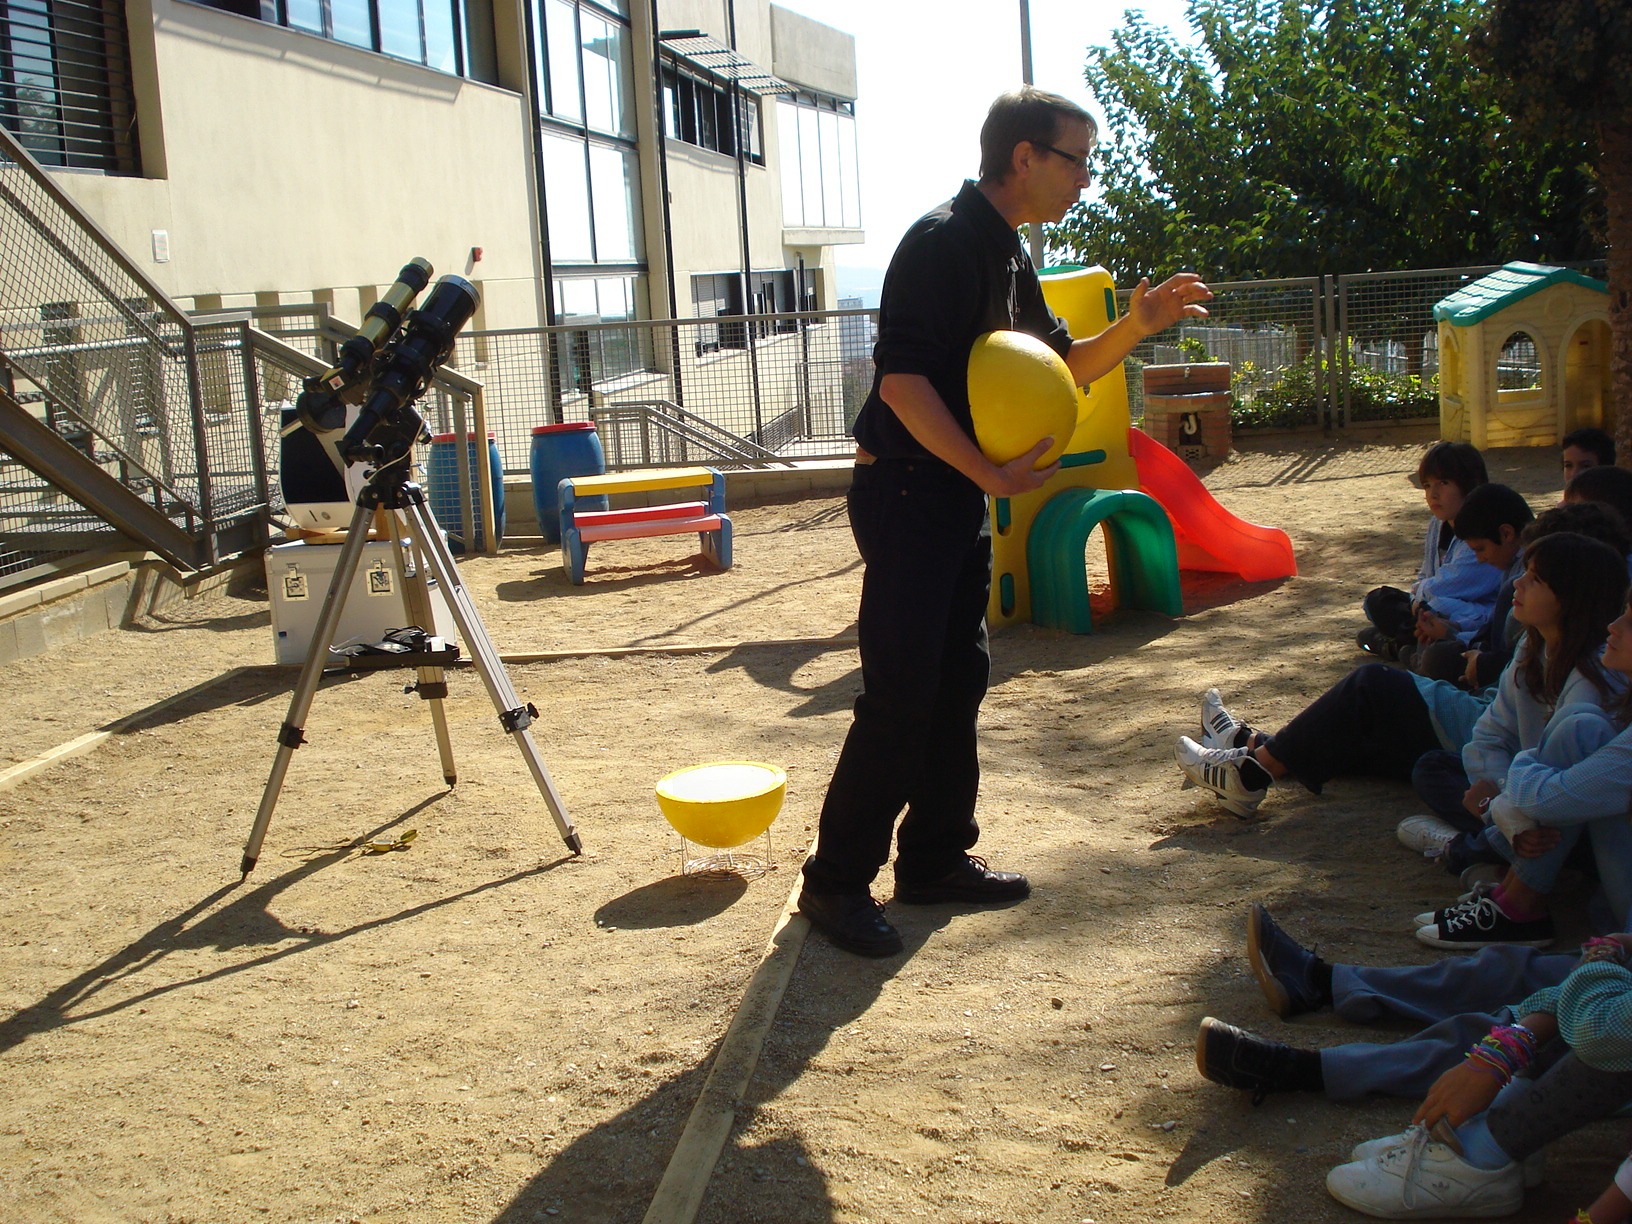
\includegraphics[width=8.5cm,keepaspectratio]{primaria/img/univers_DSC04295.JPG}}

Tots els nens i nenes de 6è vàrem pujar a una de les aules d’ESO on vam veure imatges a la pissarra digital sobre els planetes, com es va formar l’univers, els astres com el Sol,… També vam veure imatges en 3D (tres dimensions) amb unes ulleres especials. Després, vam sortir al pati de Parvulari a mirar el Sol amb un telescopi especial. Primer ens va explicar com és el Sol, els materials que té  dintre i com és que, de vegades, hi ha explosions a la seva superfície. Quan va acabar d’explicar-nos tot això, ens vam posar en fila per poder mirar pel telescopi solar. Per la primera lent del telescopi es veia el Sol com el veiem normalment, per la segona lent es veia el Sol amb el seu color real (vermell). Després vam mirar el Sol per un telescopi molt estrany que havia construït aquell astrònom. Era com una caixa de color blanc, de fusta, que tenia un telescopi  fet per ell que, al final,  hi havia un mirall que reflectia la llum del Sol a la part blanca de la caixa i es veia com el Sol es movia, però no!  El Sol en realitat no es mou, és la Terra que es mou ( jo no pensava que el moviment de la Terra fos tan ràpid!). 

\authorandplace{Aina Boronat i Marc Neira}{6è de Primària}

\end{news}

\noindent\fbox{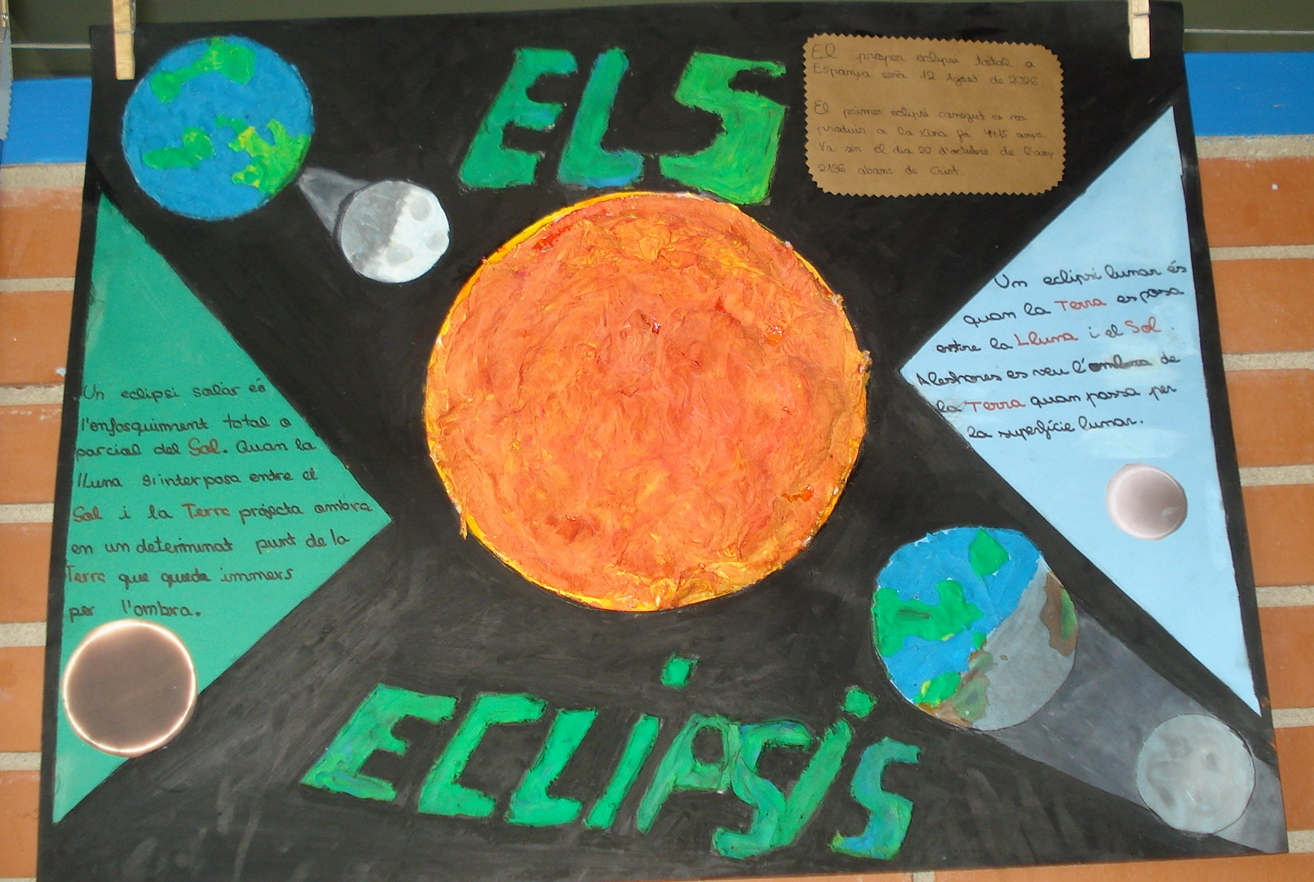
\includegraphics[width=17cm,keepaspectratio]{primaria/img/univers_DSC04296b.JPG}}

\noindent\fbox{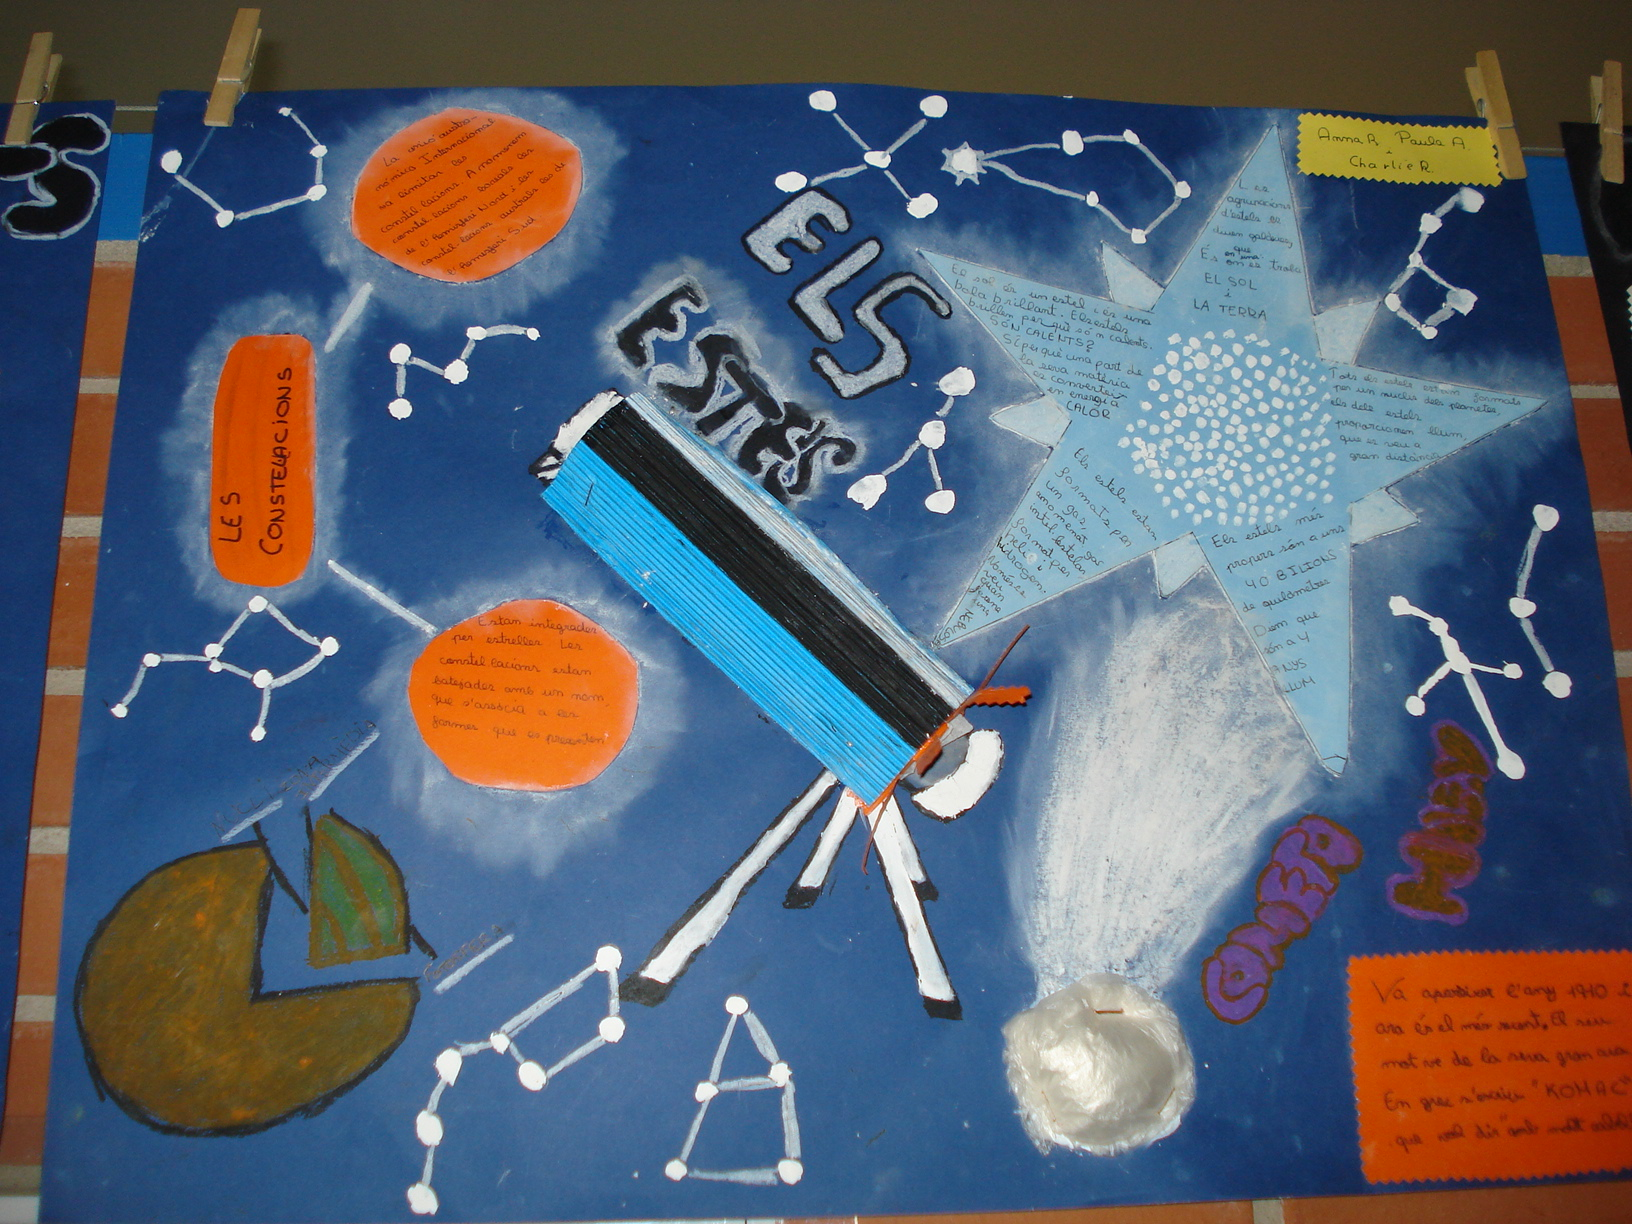
\includegraphics[width=17cm,keepaspectratio]{primaria/img/univers_DSC04300.JPG}}
  
